% !TeX root = ../thuthesis-example.tex

\chapter{引言}

\section{研究背景}
\subsection{中医药天然产物是药物发现中有价值的化学空间}

在药物发现领域,化学空间指的是通过特征和规则定义的潜在的药理学活性分子的空间,通过计算分子的特征来比对相似性,从而推测分子针对特定生物过程的活性。然而,在广阔的所有可能分子的空间中寻找有药物活性的分子是一项极具挑战性的任务。即使仅考虑符合里宾斯基五规则的小分子药物,也至少有$10^{60}$种可能的有机分子\cite{Kirkpatrick_Ellis_2004},这对实际的药物筛选是不可接受的。在现有的药物发现流程中,往往使用虚拟筛选方法,包括基于结构的药物设计和基于配体的药物设计。其中,前者要求具体的目标蛋白结构,需要首先根据生物学研究范式确定目标靶点,后者通过计算分子之间的相似性进行预测,但是结构相似性和生物活性之间的关系并不强烈甚至并不明确。因此,在这些方法的基础上,我们可能需要更多的先验来指导药物发现的探索过程,利用我国传统中草药的丰富资源就是一条可行的途径。一方面,中草药来自种类繁多的植物,其天然产物构成一个广阔的化学空间,为药物发现提供了搜索范围;另一方面,许多中草药的药理活性已经在中医药几千年的临床实践中得到验证,这些前人总结出的经验显示了中草药天然产物相比随机分子显著更高的成药可能。\cite{发挥我国传统医药及资源优势进行创新药物的基础研究}因此,以中草药天然产物为基础,可以为药物发现提供更多的先验知识。

相比传统基于单个候选分子与靶点作用的药物发现方法,从中草药出发进行探索还具有整体性、系统性的特点。中医药的理论与实践并不总是进行单一有效成分的提取、纯化和使用,而是将多种药材结合使用,形成“方剂”,有意让多种有效成分协同发挥作用。\cite{张彦琼:883}从现代生物学的角度看,中药方剂在发挥药效时,其中的多种有效成分可能作用于不同的靶点,从而在生物体内形成复杂的网络效应,整体对特定信号通路、生物过程产生调控作用。因此,从中草药出发进行药物发现,可以更好地利用这种调控网络的整体性、系统性,从而更好地发现临床意义上的新药。

\subsection{中药组成数据的定量}

中草药组成成分的确定和定量是新药研发中的重要一环。有了充足的定量数据,我们才得以比较药材成分,进行高通量筛选,应用统计学和机器学习方法寻找相关性,从而确定候选药材和分子。作为多组分天然产物,中草药的成分分析方法主要包括色谱法、质谱法、核磁共振法等。\cite{中药有效部位及成分提取工艺和检测方法_2007}在质量检测、产地溯源等实际应用的驱动下,已经形成了对特定中药材的检测仪器技术。然而,这一步骤并不容易。一方面,中草药的组成成分种类繁多,而同一药材在不同的生长环境下,其成分与含量也可能有所不同,这是问题本身的复杂性;另一方面,关于中草药的定量研究起步晚、规模小,而进行定量研究的成本高昂,效率较低,导致全国乃至世界范围内尚未形成统一的标准和完善的数据库。如下统计图\ref{fig:statistics}所示,现有的中医药数据库具有分散程度高、单个规模小,信息组织不够结构化的问题,这给中草药的定量研究带来了挑战。\cite{Yang_Zhu_Yao_Chen_Chen_Gu_Jiang_Chen_Zhang_Wu_et_al._2023}

\begin{figure}[H]
  \centering
  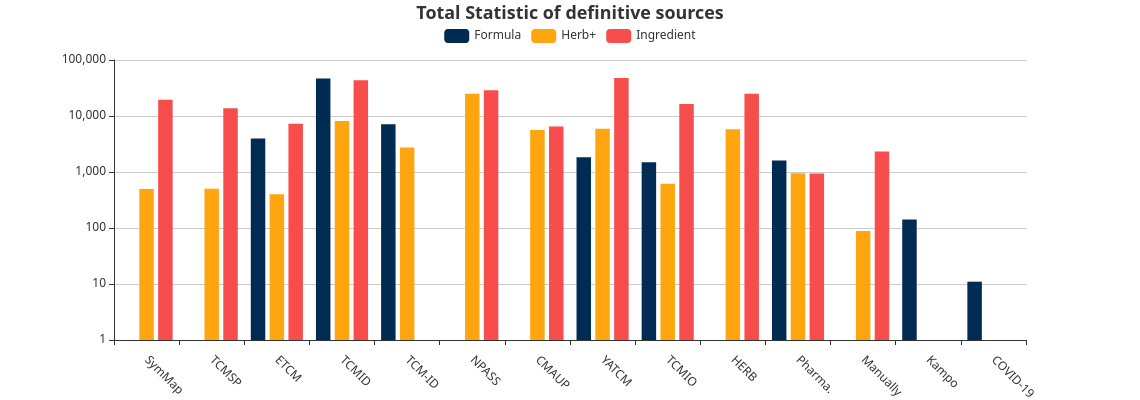
\includegraphics[width=\linewidth]{total_statistic_of_definitiv_sources.png}
  \caption{现有中药数据库的统计信息}
  \label{fig:statistics}
\end{figure}


为了应对这一挑战,除了期望中药数据库的发展完善外,我们可以通过主动收集数据和优化处理方法的方式进行解决。其中,主动收集数据包括对研究中重点关注的中草药进行直接定量分析,以及对已有的中草药成分定量数据进行整理、收集和标准化,从而形成一个可供后续研究使用的数据库。优化处理方法则包括选用合适的建模方法,如非参数统计方法、集成学习、迁移学习,或者利用先验补足数据的缺失,建立概率图模型来更好地利用有限的数据。此外,我们还可以使用临床实验数据和基于分子对接的计算方法来辅助中草药成分的定量研究。

\section{研究现状}

\subsection{中药靶点预测任务}

在中药组成数据的基础上,我们可以进行多种下游任务,如中药靶点预测、传统理论属性解释、中药剂量关系,乃至处方优化等。其中,本课题的重点是中药靶点预测。如果确定了针对某种具体疾病或表征有显著效果的天然产物分子,我们可以,通过直接查询已有的靶点数据库,进行化学相似性搜索、反向药效团搜索,或者应用反向分子对接的方法,利用三维建模测试分子与靶点的亲和力,从而预测分子的靶点。\cite{Huang_Zhang_Zhou_Lin_Chen_Lin_Mai_Huang_2018}然而,在更多的情形中,我们无法确定具体的药效分子,往往需要建立复杂的药物-靶点互作网络。面对中药相关数据量有限的问题,我们还可以进行药物-基因-疾病关联分析,建立概率图模型,将药物作用靶点建模成隐变量,通过这种一体化分析方法提高预测能力。目前,中药网络药理学的最新重要参考是本草组鉴(HERB)数据库,基于文本挖掘,辅以人工标定,结合数据库掘和统计推断,共将12,933个靶点28,212种疾病和7,263种中草药、49,258种成分联系起来,并提供了它们之间的六种配对关系。其中部分提供高通量实验证据、差异分析及富集分析结果。\cite{Fang_Dong_Liu_Guo_Zhao_Zhang_Bu_Liu_Huo_Cao_et_al._2021}这将是我们后续分析过程中的有力支撑。

\begin{figure}[H]
  \centering
  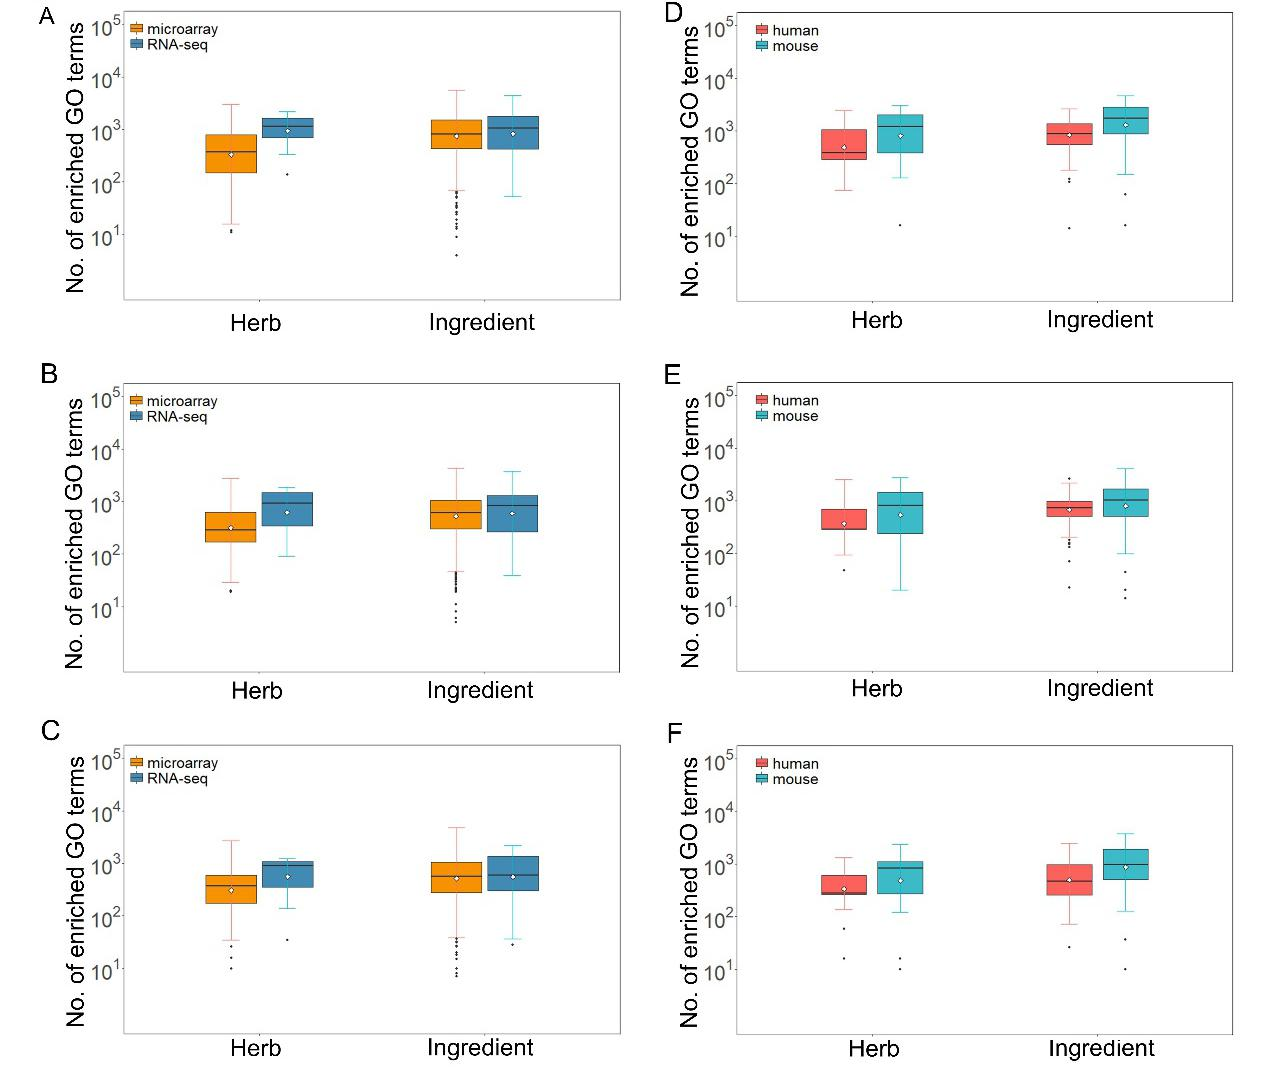
\includegraphics[width=\linewidth]{figures/HERB.png}
  \caption{HERB数据库提供的六种配对关系,其中ABC/DEF分别基于微观/宏观实践结果,而AD/BE/CF分别展示差异/上调/下调基因\cite{Fang_Dong_Liu_Guo_Zhao_Zhang_Bu_Liu_Huo_Cao_et_al._2021}}
  \label{fig:HERB}
\end{figure}

\subsection{现有的靶标预测算法}

\subsubsection{基于分子指纹的结构相似性算法}

分子指纹是一种分子抽象表征的方法,通过一定的规则将分子由二维结构图压缩为一维比特向量。在恰当的映射方式下,分子指纹的公共片段可以表征原分子的局部结构相似性,从而将二维分子的比较转化为可在计算机中高效处理的一维向量比较。使用基于分子指纹的结构相似性算法进行靶标预测,就是在已有数据库的靶点配体分子中寻找与待预测分子结构相似的分子进行预测。根据分子指纹的生成方式,可以定义一系列的算法并建立相应数据库,如基于拓扑结构的Daylight分子指纹对应SEA数据库\cite{Keiser_Roth_Armbruster_Ernsberger_Irwin_Shoichet_2007},基于圆形子结构的ECFP分子指纹对应SuperPred数据库\cite{Nickel_Gohlke_Erehman_Banerjee_Rong_Goede_Dunkel_Preissner_2014}。这些算法在小分子预测任务上不断进行迭代开发,目前已经取得了较好的效果。

\subsubsection{多重相似性算法}

然而,上述基于化学结构的方法中的假设并不普遍正确,结构相似的药物可能结合无明显结构、序列相似性的靶点,而结构细节的微小差异就有可能造成对同一靶点截然不同的结合能力,这在分子对接中是可以验证的结论。因此,除了结构信息外,我们还可以引入基因表达上下游的其他信息,通过整合后的信息进行更加准确的判断。其中的一个典型代表是drugCIPHER-MS算法。在药理学空间内,这种方法在化学相似性(CS)之外从下游表型定义了一个治疗相似性(TS);除此以外,还引入了靶标蛋白质相关性的蛋白质-蛋白质相互作用(PPI)网络特征,从而建立了一个高维回归模型,充分整合各个层面的已知信息,从而提高了预测的准确性。\cite{Zhao_Li_2010}

\begin{figure}[H]
  \centering
  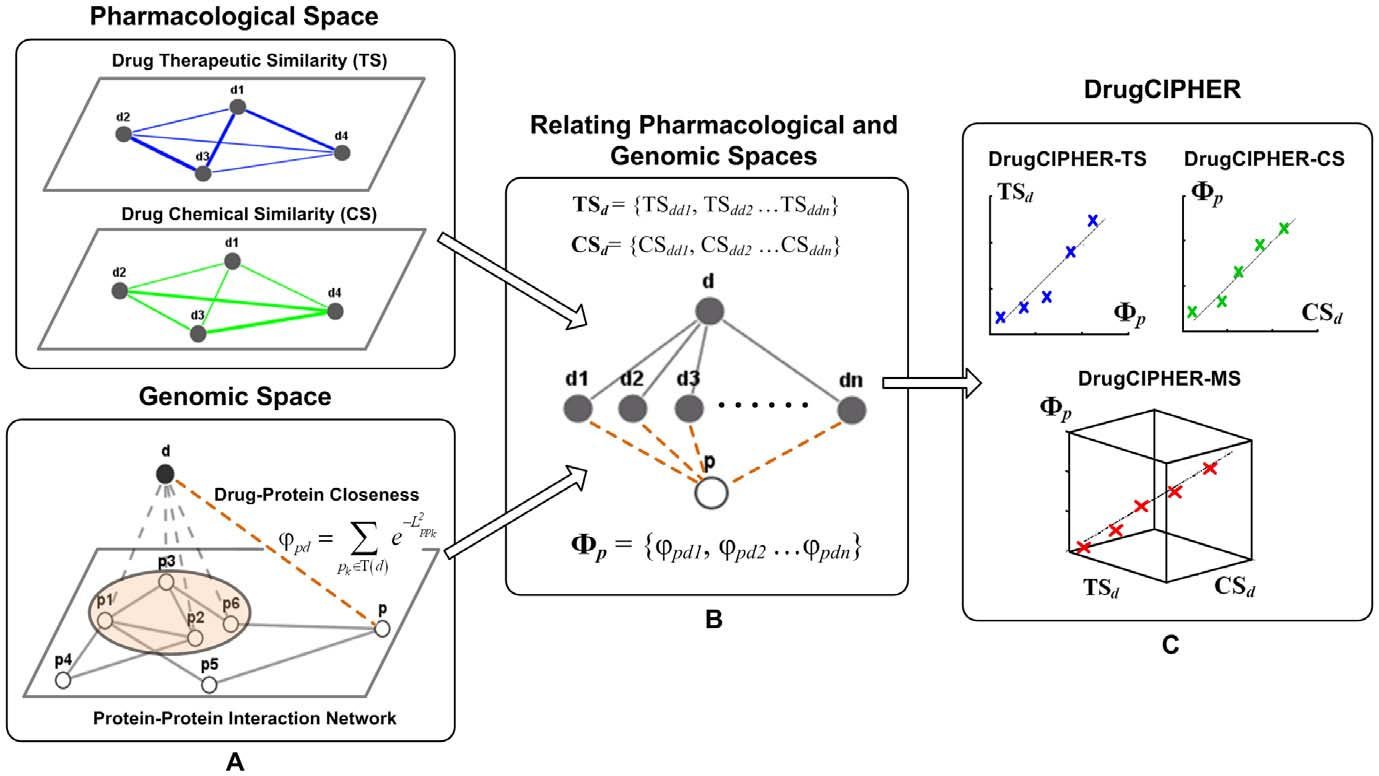
\includegraphics[width=\linewidth]{figures/drugCIPHER-MS.png}
  \caption{drugCIPHER-MS算法原理\cite{Zhao_Li_2010}}
  \label{fig:drugCIPHER-MS}
\end{figure}

\subsection{深度学习方案在中药靶点预测中应用的可能}

在目前的药物靶点预测中,利用深度学习的方法进行预测已经取得了显著的成果。应用在药物靶点预测中的深度学习方法主要包括卷积神经网络(CNN)、图神经网络(GNN)等\cite{Tsubaki_Tomii_Sese_2019},可以有效解决数据集不平衡、标记数据少而未标记数据多等情形下的问题,显著提高预测的准确性和稳定性。事实上,深度学习模型并不是取代了上述的靶标预测算法,而是将它们的思想作为学习中的损失函数,网络拓扑等信息,同样利用好了已有的信息和建模。此外,深度学习中的循环神经网络(RNN),长短期记忆网络(LSTM)等结构,乃至Transformer,BERT和GPT等生成式深度学习模型正逐步取得关注和应用。这些模型在具体任务间具有强大的迁移能力,已经在自然语言处理、计算机视觉等领域取得了众多显著的成果,且已在药物发现领域取得了初步的应用,因此我们有理由相信他们在靶点预测乃至整个药物-靶点-疾病网络预测中也会发挥重要作用。\cite{Haroon_C.a._A.s._2023}

以上所述进展大多为小分子药物,有一些也迁移到抗蛋白质-蛋白质结合等领域,但总体而言,中药靶点预测的深度学习方法尚未有较为系统的研究。因此,我们认为,将深度学习方法应用于中药靶点预测,将会是一个有意义的尝试。

\subsection{中药靶点预测的实验验证}

在通过上述预测方法确定了药物靶点后,可以通过实验方法加以验证。对于涉及一个或少数靶点的药物,可以通过基因敲除的方法直接验证,从而证明药物作用的机制;然而,在中药的情形下,也有可能出现药物作用于多个靶点,对调控网络施加整体影响的效果。针对这种情况,可能的思路有使用CRISPR/Cas9\cite{Cong_Ran_Cox_Lin_Barretto_Habib_Hsu_Wu_Jiang_Marraffini_et_al._2013}技术进行多靶点的敲除,或者使用dCas9\cite{Jiang_Geng_Wang_Liang_Guo_Liu_Zhao_Jin_Liu_Mu_2023}、RNAi\cite{Zimmermann_Lehár_Keith_2007}等技术进行多靶点的抑制,从而验证药物的作用机制,并结合基因表达谱的变化进行更全面完善的分析。
